%-*- coding:utf-8 -*-

\title{ALPSチュートリアル -- アプリケーション実習(2)}

\begin{document}

\lstset{language={C++},showspaces=false,rulecolor=\color[cmyk]{0, 0.29,0.84,0}}

\begin{frame}
  \titlepage
\end{frame}

\section*{Outline}
\begin{frame}[t,fragile]
   \tableofcontents
\end{frame}

\section{ALPSシミュレーションの流れ}

\subsection*{\redm\whiteb\greenb}
\begin{frame}{ALPSシミュレーションのワークフロー}
  \begin{center}
    \includegraphics[height=0.8\textheight]{workflow.pdf}
  \end{center}
\end{frame}

\subsection*{\redm\whiteb\greenb}
\begin{frame}[t,fragile]
  \frametitle{ALPSシミュレーションの実行例}
  \begin{itemize}
    \item Pythonからのシミュレーションの実行
\begin{lstlisting}
$ cd $HOME/tutorials/mc-02-susceptibilities
$ python tutorial2a.py
$ python tutorial2b.py
$ python tutorial2c.py
$ python tutorial2d.py
$ python tutorial2full.py
\end{lstlisting}
    \item Pythonスクリプトを実行するたびに、結果のグラフが表示される
    \item グラフのウィンドウを閉じるとスクリプトは終了
    \item 最後のスクリプトは、全ての計算結果を一枚のグラフに表示
  \end{itemize}
\end{frame}

\subsection*{\redm\whiteb\greenb}
\begin{frame}[t,fragile]
  \frametitle{いったい何を計算したの?}
  \begin{itemize}
  \item 様々な反強磁性ハイゼンベルグ模型の帯磁率の温度依存性
    \begin{itemize}
    \item tutorial2a.py: 古典ハイゼンベルグ模型(一次元鎖)
    \item tutorial2b.py: 古典ハイゼンベルグ模型(二本足はしご)
    \item tutorial2c.py: $S=1/2$古典ハイゼンベルグ模型(一次元鎖)
    \item tutorial2d.py: $S=1/2$量子ハイゼンベルグ模型(二本足はしご)
    \end{itemize}
  \item 問題
    \begin{itemize}
      \item 古典系と量子系とふるまいの違い
      \item 格子構造による帯磁率のふるまいの違い
      \item 帯磁率のふるまいの違いの原因は?
    \end{itemize}
  \end{itemize}
\end{frame}

\section{入力ファイルの準備}

\subsection*{\redm\whiteb\greenb}
\begin{frame}{ALPSシミュレーションの入出力}
  \begin{itemize}
  \item 典型的には、一つのシミュレーションは複数のパラメータセットからなる(異なる温度など)
    \begin{itemize}
    \item 「ジョブ(job)」: シミュレーション全体、「タスク」の集合
    \item 「タスク(task)」(または「simulation」):– 一つのパラメータセットに対する計算、「ラン」の集合
    \item 「ラン(run)」(または「clone」): 異なる乱数の種に対する個々の計算
    \end{itemize}
  \item XML入力ファイルと出力ファイル
  \begin{center}
    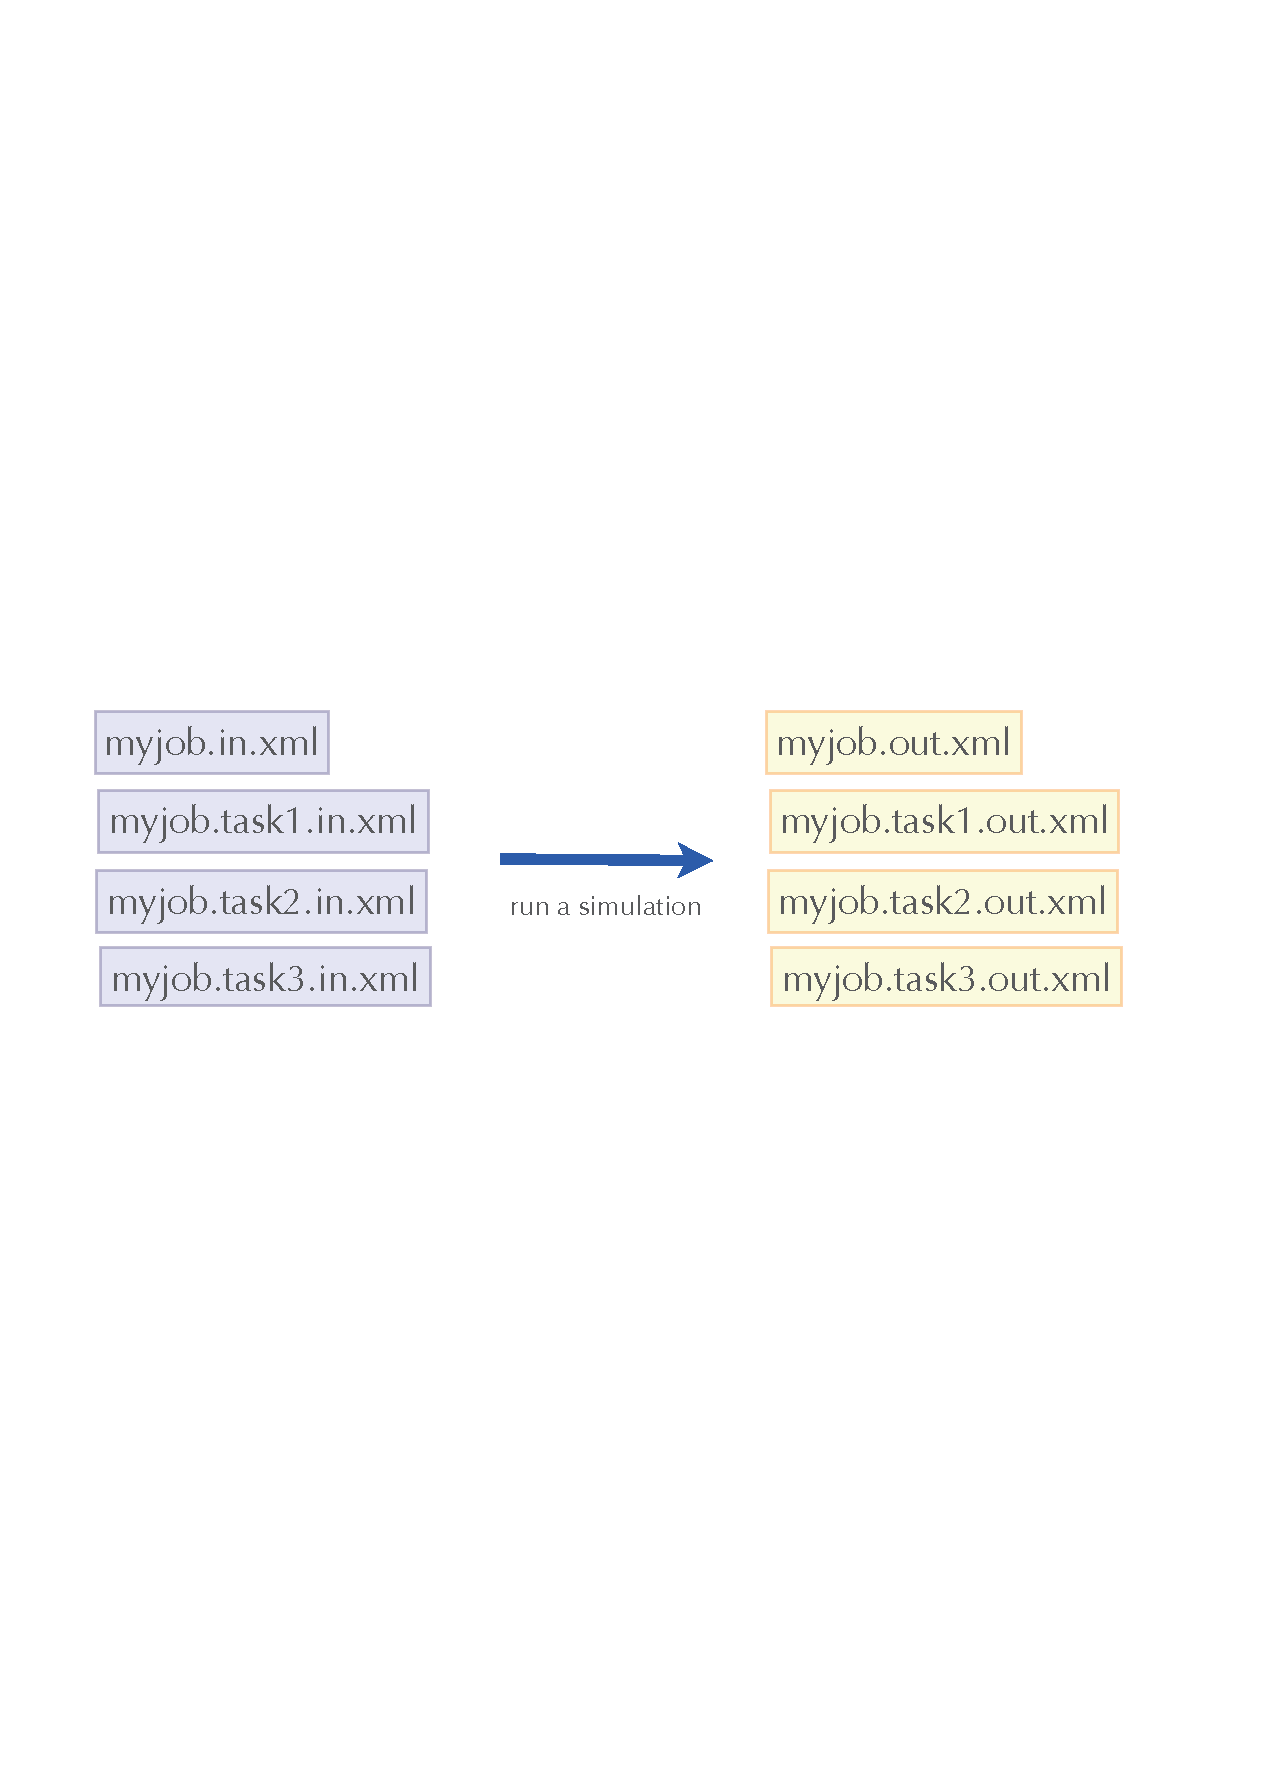
\includegraphics[width=.55\textwidth]{simulation1.pdf}
  \end{center}
  \end{itemize}
\end{frame}

\subsection*{\redm\whitem\greenb}
\begin{frame}{XMLの基礎}
  \begin{itemize}
  \item XML = e{\color{red} X}tensible {\color{red} M}arckup {\color{red} L}anduage
  \item 構造化文書を作成するのに適している
  \item 「タグ」を使って、文章の構造を記述
  \item 大文字と小文字は区別される
  \item XMLの例: HTML (XHTML)
  \begin{center}
    \includegraphics[height=0.3\textheight]{xml1.pdf}
  \end{center}
  \end{itemize}
\end{frame}

\subsection*{\redm\whitem\greenb}
\begin{frame}{XMLの文法}
  \begin{itemize}
  \item 「開始タグ」には対応する「終了タグ」が必要
  \item ある要素の「開始タグ」と終了タグは共通の親ノードに含まれなければならない
  \item XMLの「木」表示
  \begin{center}
    \includegraphics[width=\textwidth]{xml2.pdf}
  \end{center}
  \item XMLでは、ユーザが独自のタグ(要素の名前)を定義することが可能 (参考: Document Type Definition (DTD), XML Schema)
  \end{itemize}
\end{frame}

\subsection*{\redm\whitem\greenb}
\begin{frame}{なぜXMLを使うのか?}
  \begin{center}
    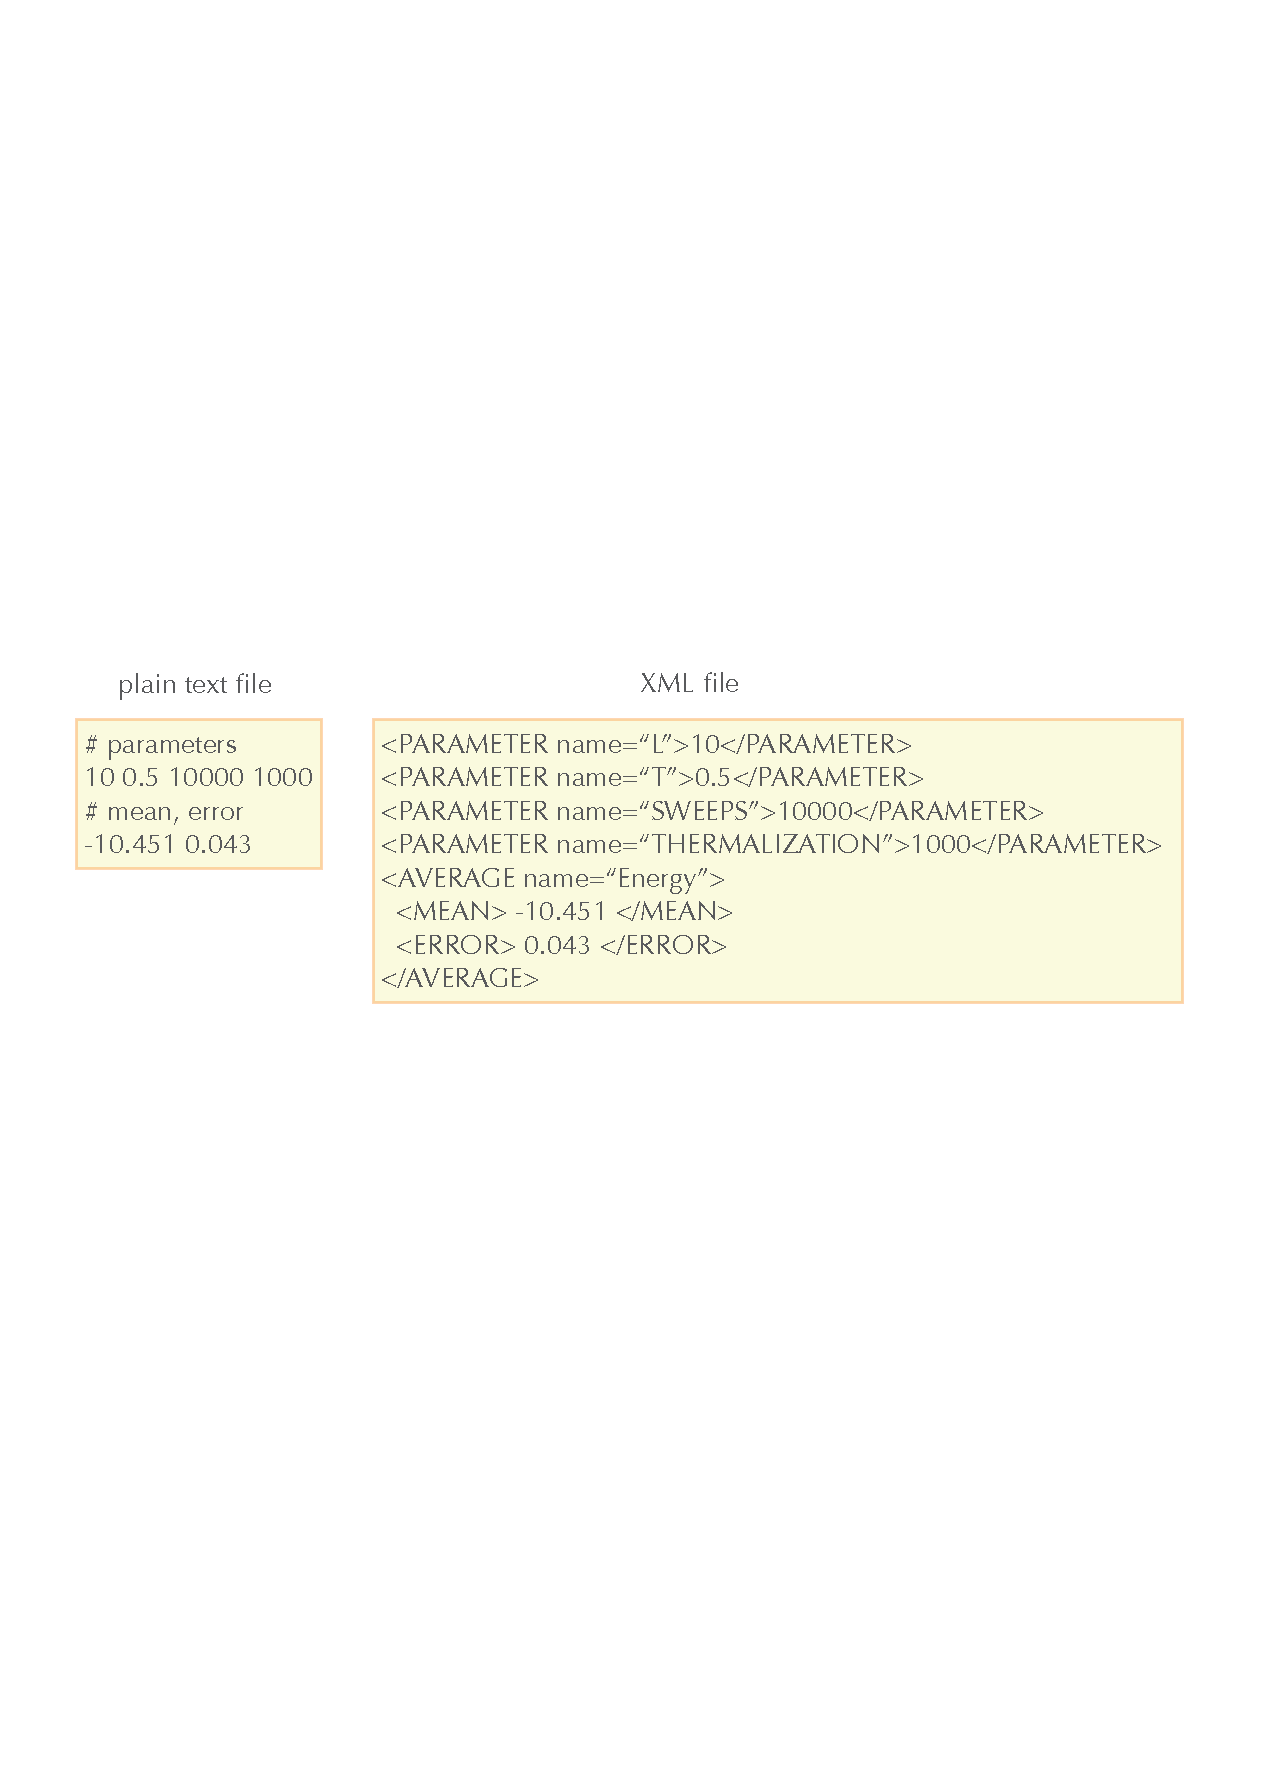
\includegraphics[width=.8\textwidth]{xml3.pdf}
  \end{center}
  \begin{itemize}
  \item 人間にはどちらが読みやすい?
  \item 機械にはどちらがよみやすい?
  \item 数年後に読んで理解できるのはどっち?
  \end{itemize}
\end{frame}

\subsection*{\redm\whitem\greenb}
\begin{frame}{データ形式の拡張性}
  \begin{itemize}
  \item 新しいパラメータを追加すると、、、
  \begin{center}
    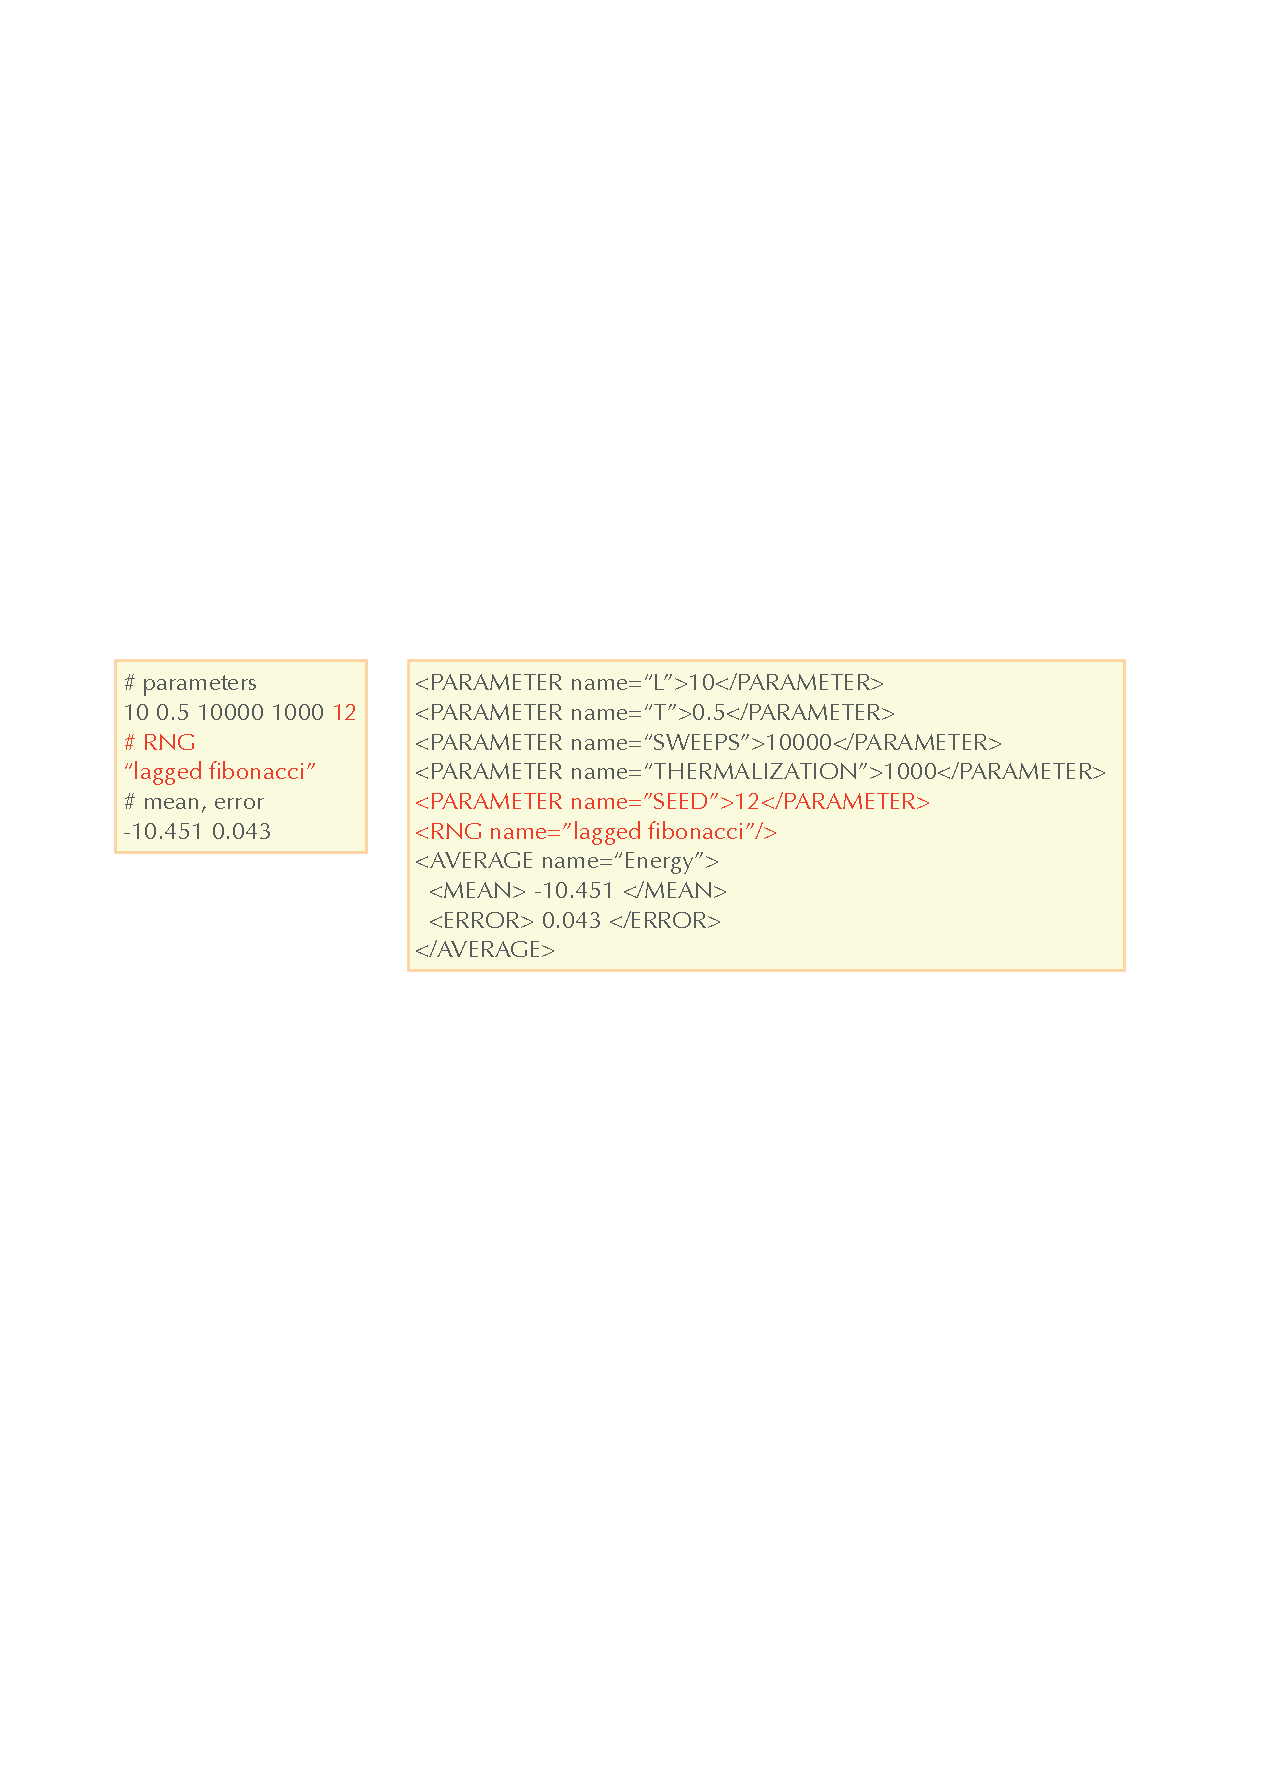
\includegraphics[width=.8\textwidth]{xml4.pdf}
  \end{center}
  \item テキスト形式の場合、これまでのプログラムは動かなくなる
  \item XMLの場合には問題ない (必要のないパラメータは読まれない)
  \end{itemize}
\end{frame}

\subsection*{\redm\whiteb\greenb}
\begin{frame}{Job XML ファイル(マスターファイル)}
  \begin{center}
    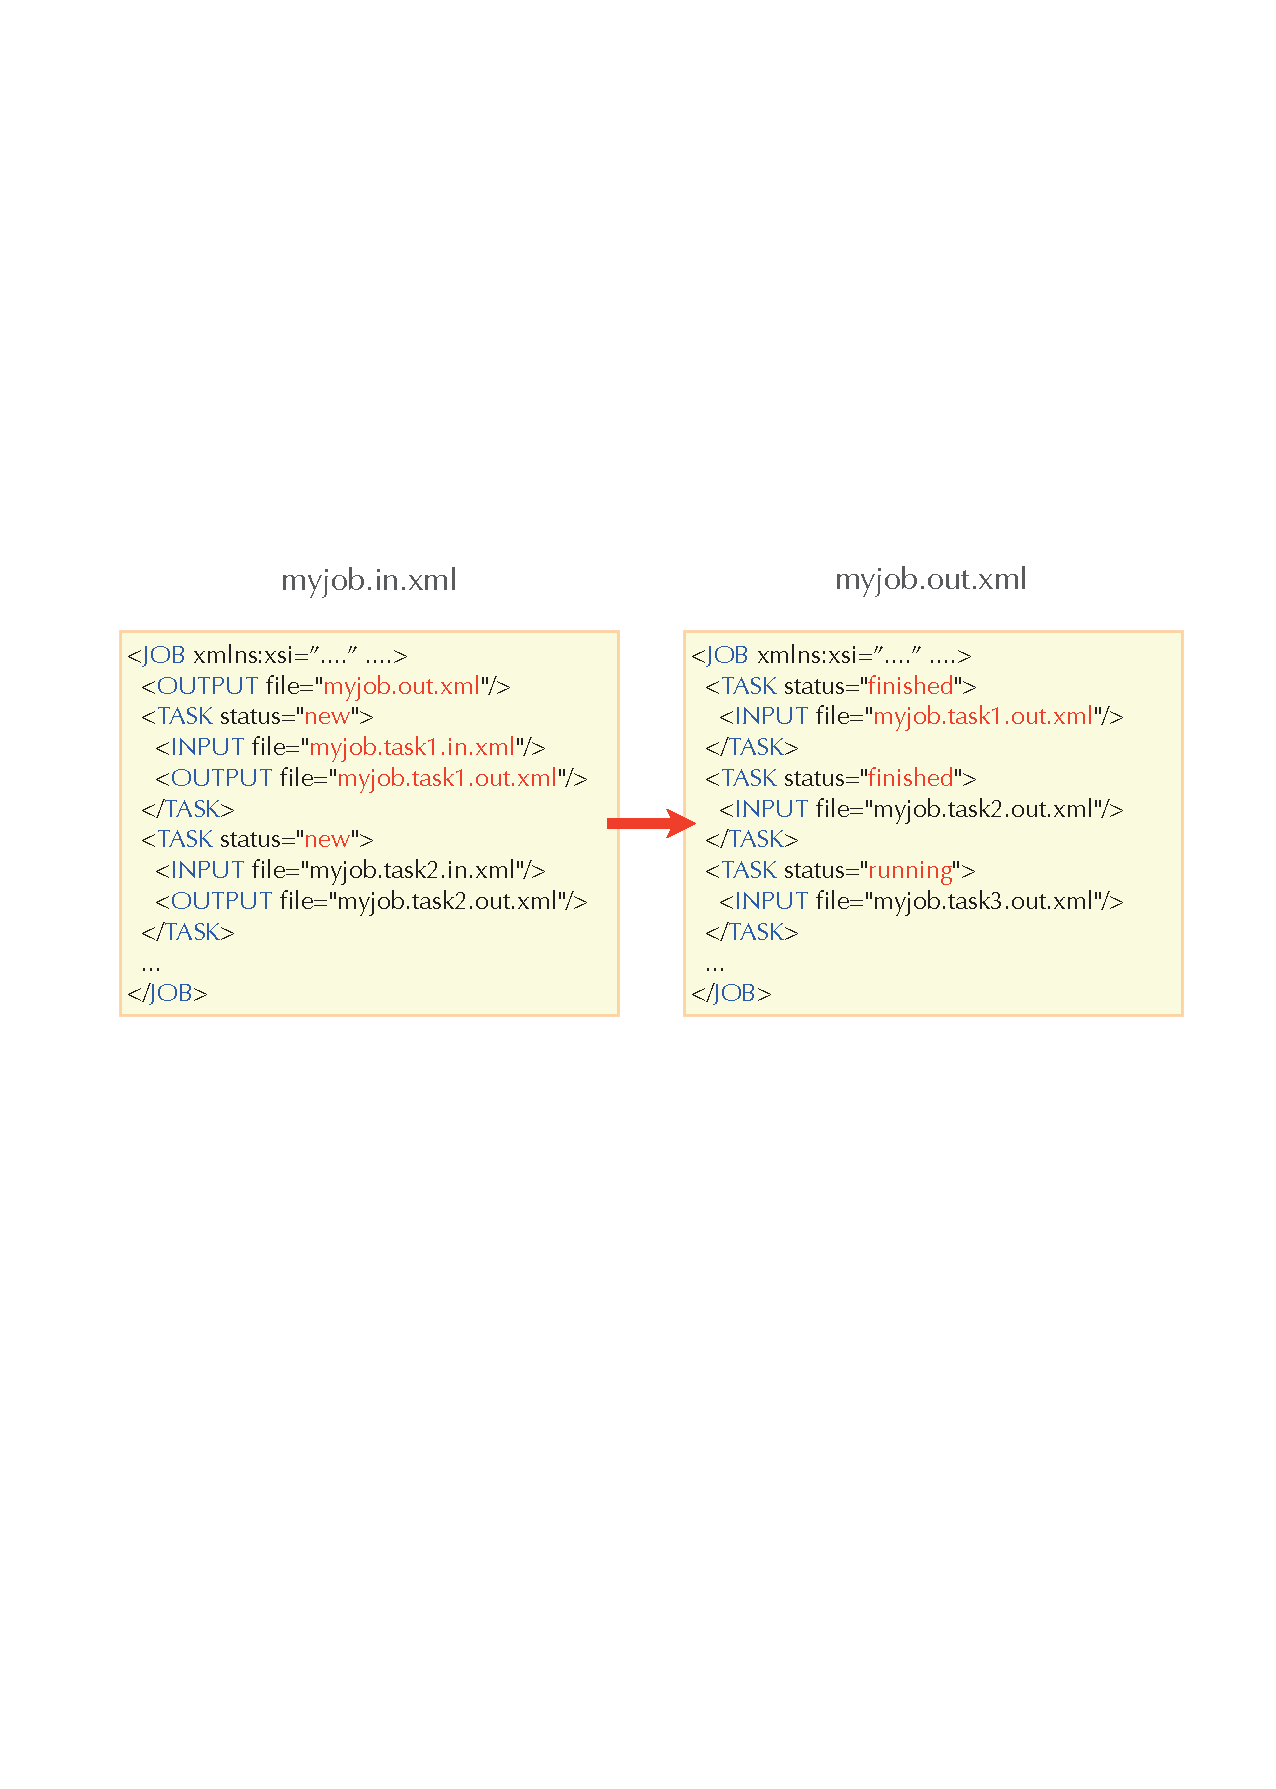
\includegraphics[height=.6\textheight]{simulation2.pdf}
  \end{center}
\end{frame}

\subsection*{\redm\whiteb\greenb}
\begin{frame}{Task XML ファイル}
  \begin{center}
    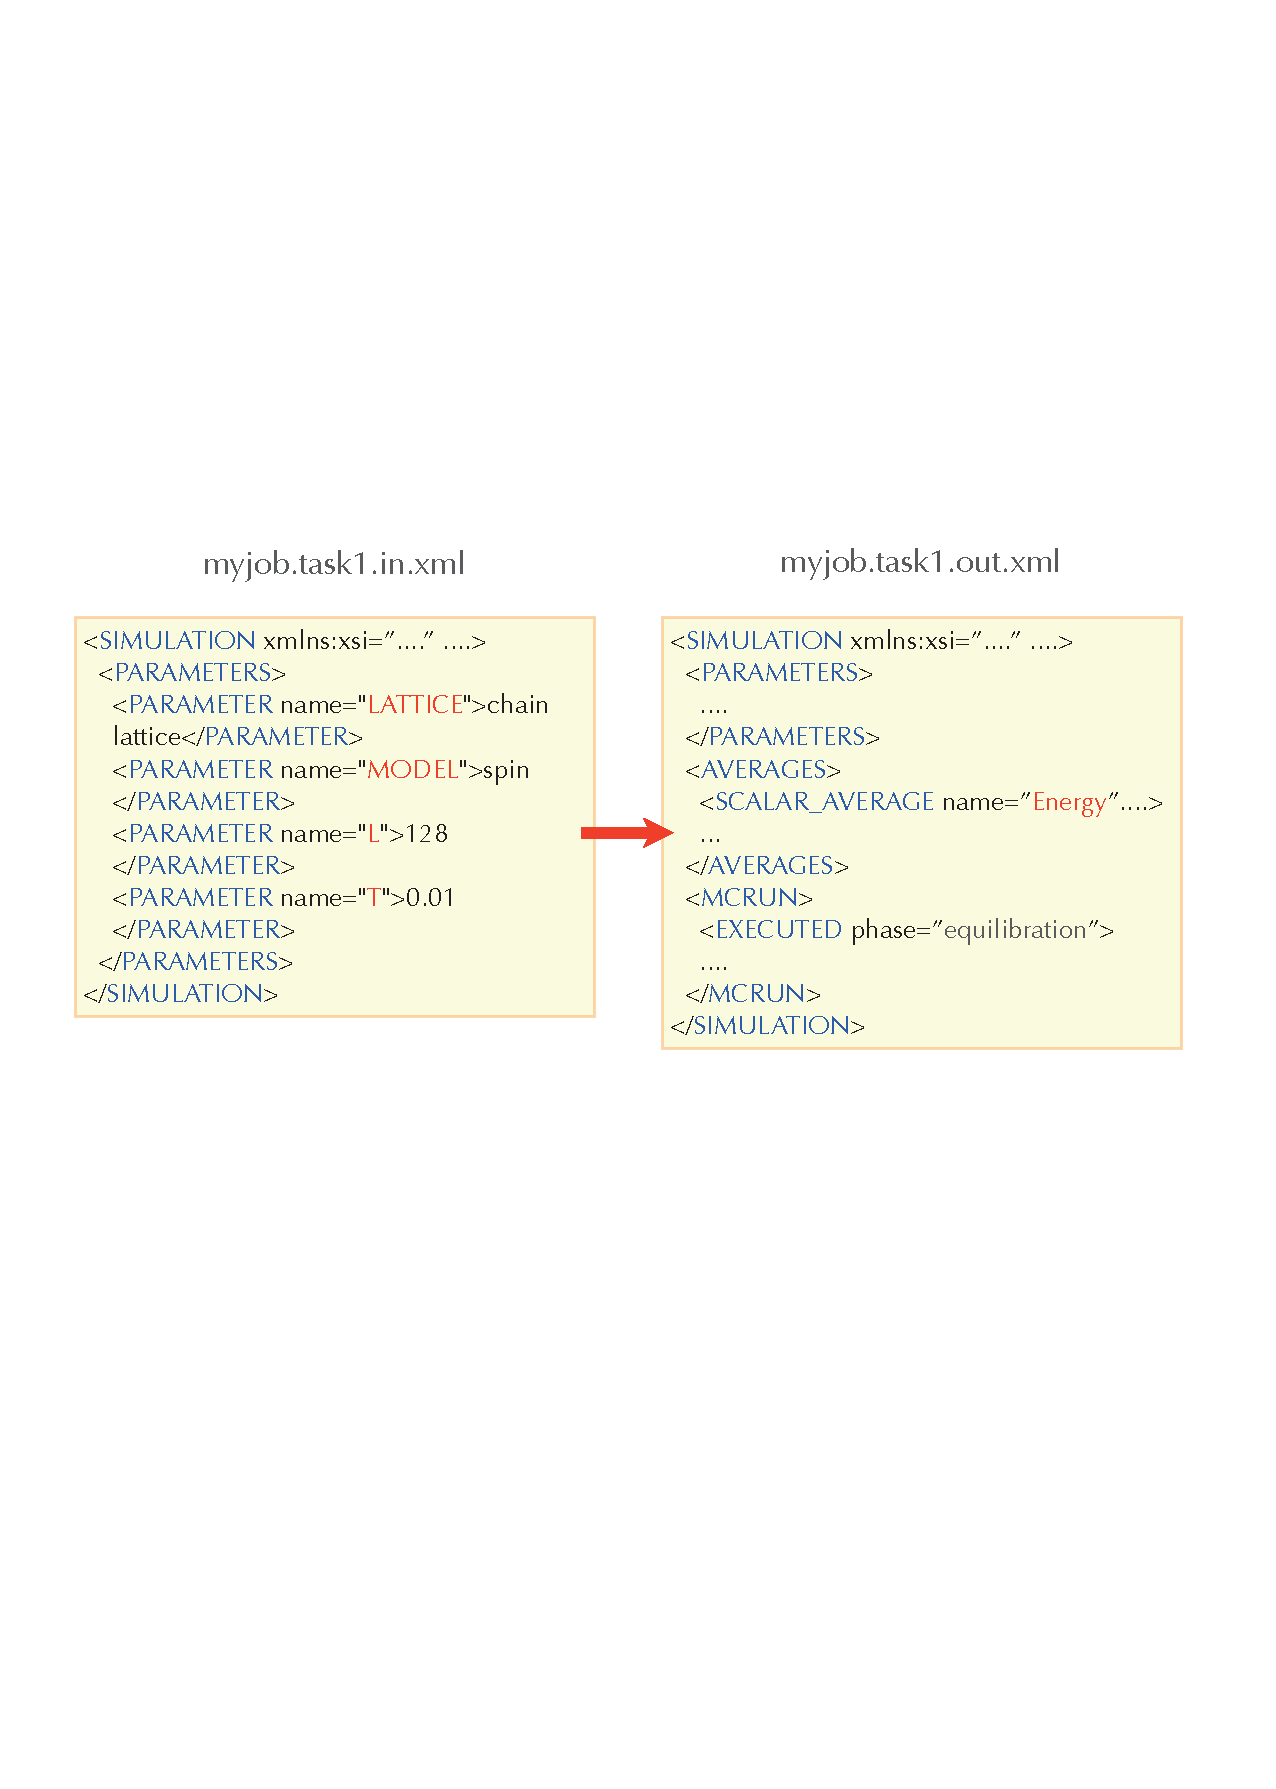
\includegraphics[height=.6\textheight]{simulation3.pdf}
  \end{center}
\end{frame}

\subsection*{\redm\whiteb\greenb}
\begin{frame}{ALPSによって生成されるバイナリ形式ファイル}
  \begin{itemize}
    \setlength{\itemsep}{1em}
  \item HDF5 (拡張子 {.h5})
    \begin{itemize}
    \item 実行結果や実行時情報は, Task毎にHDF5形式ファイルに保存される
    \item pyalpsツールは, HDF5ファイルから計算結果を読み込む
    \end{itemize}
  \item XDR (拡張子 {.xdr})
    \begin{itemize}
    \item 実行途中のチェックポイント情報(スピン配位等)が定期的に保存される
    \item シミュレーションのリスタート時は, 最後のチェックポイントから再開される
    \end{itemize}
  \end{itemize}
\end{frame}

\subsection*{\redm\whiteb\greenb}
\begin{frame}[t,fragile]{入力ファイルの準備}
  \begin{enumerate}
    \setlength{\itemsep}{1em}
  \item Pythonスクリプトによる生成: 例) \href{https://github.com/cmsi/alps-tutorial/blob/tutorials/tutorials/mc-02-susceptibilities/tutorial2a.py}{tutorial2a.py}
    %\begin{center}
      \includegraphics[height=.72\textheight]{tutorial2a-1.pdf}
    %\end{center}
  \end{enumerate}
\end{frame}

\subsection*{\redm\whiteb\greenb}
\begin{frame}[t,fragile]{入力ファイルの準備}
  \begin{enumerate}
    \setlength{\itemsep}{1em}
    \setcounter{enumi}{1}
  \item 簡易テキスト形式で作成し、{\tt parameter2xml}ツールでXMLに変換: 例) parameter2xml myjob
    \begin{center}
      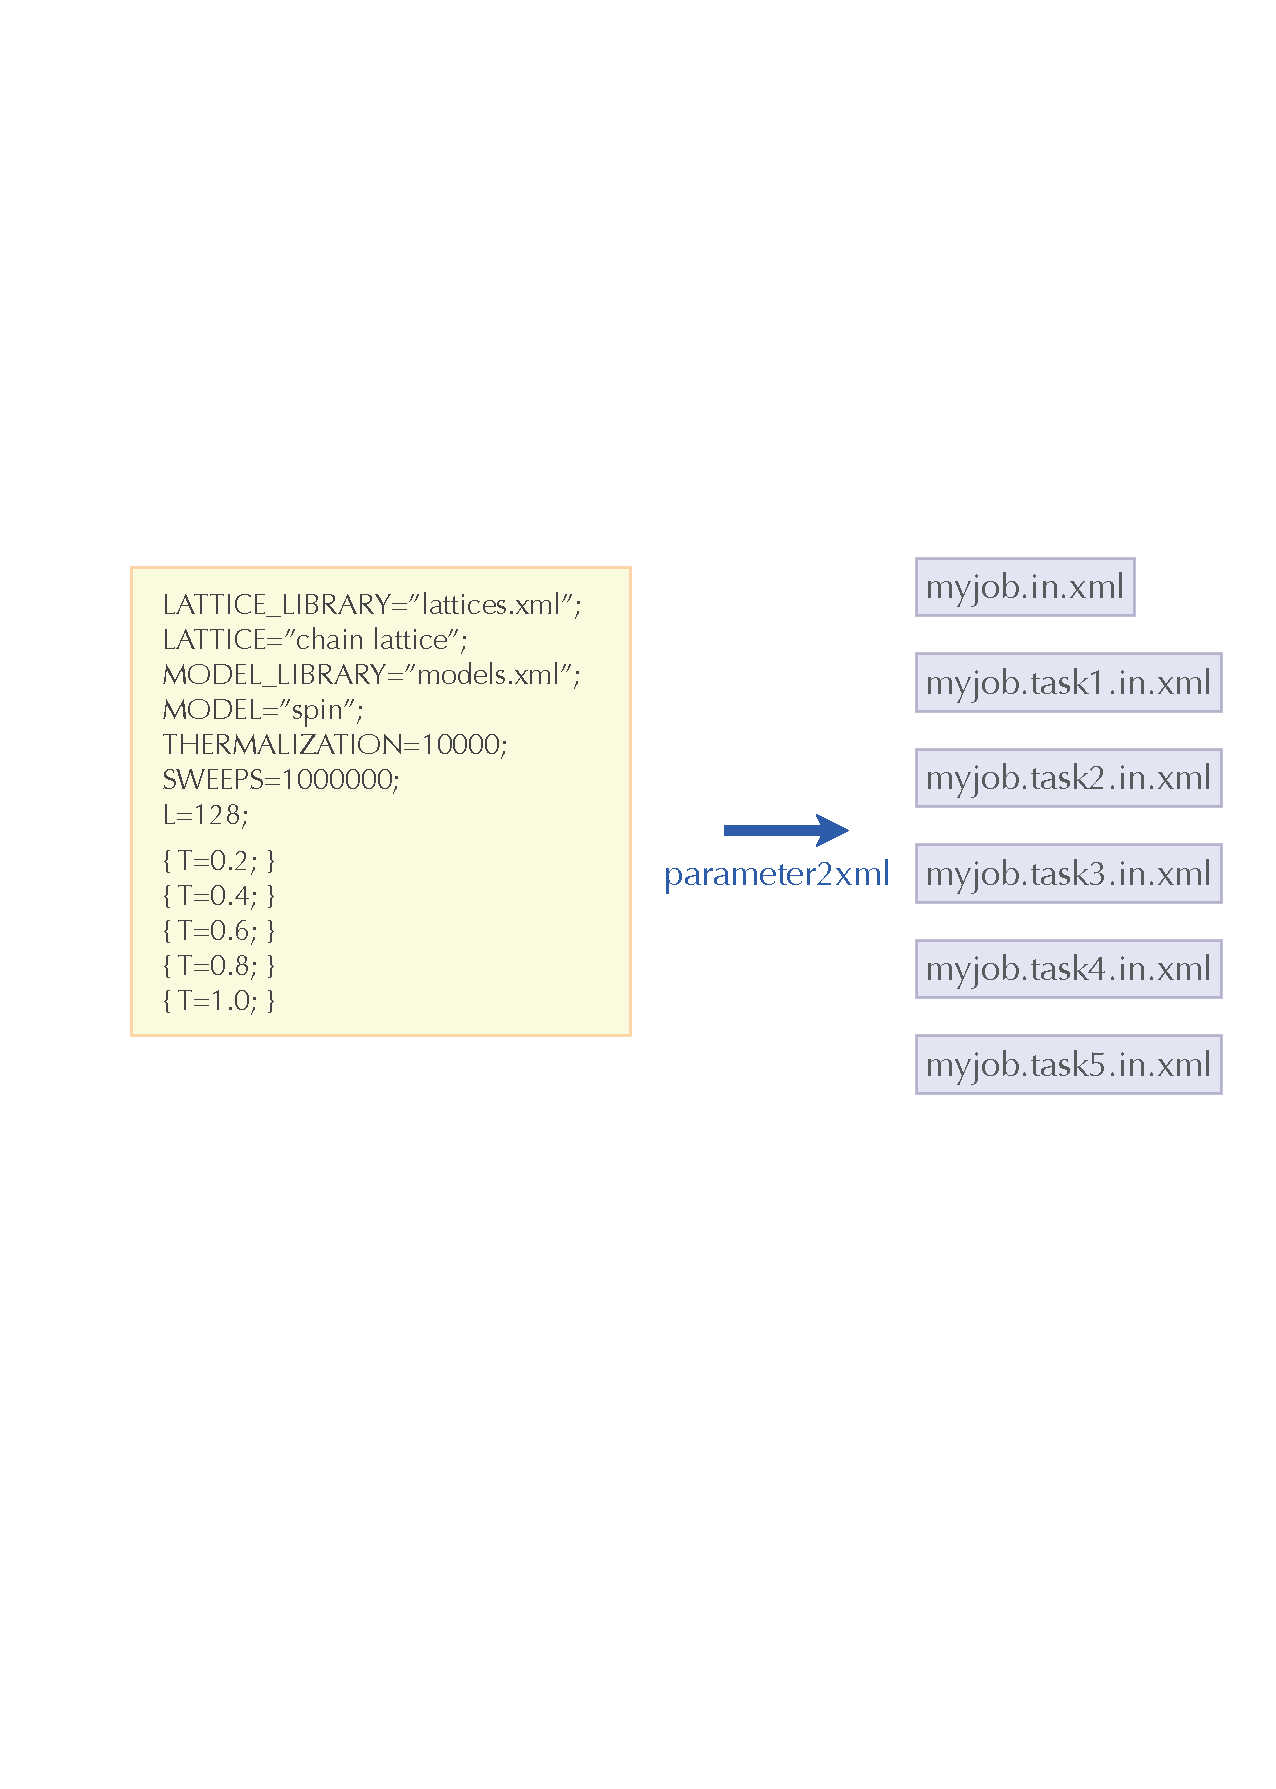
\includegraphics[height=.6\textheight]{simulation4.pdf}
    \end{center}
  \end{enumerate}
\end{frame}

\subsection*{\redm\whiteb\greenb}
\begin{frame}[t,fragile]
  \frametitle{Simplified parameter file format}
  \begin{columns}[T]
    \begin{column}{.5\textwidth}
      \begin{itemize}
        %\begin{itemize}
        \item 改行、セミコロン、コンマで変数を区別
        \item \{ \}で囲んだ変数は異なるパラメータセット
        \item \{ \}の前の変数は共通パラメータ
        \item $\pi$ (PI), 虚数単位(I)
        \item C 風, C++風のコメント
        \item 「循環参照」がある場合にはエラーとなる
        %\end{itemize}
      \end{itemize}
    \end{column}
    \begin{column}{.5\textwidth}
    \begin{lstlisting}
LATTICE = "chain lattice";
L = 16,
SEED = 2873
// C++ style comment
SWEEPS = 4096;
THERMALIZATION = SWEEPS/8;
/* C style comment */
{ T = 2; Sq = 2*PI/3; }
{ T = 1.8; }
    \end{lstlisting}
    \end{column}
  \end{columns}
\end{frame}

\subsection*{\redm\whiteb\greenb}
\begin{frame}{格子とモデルの指定}
  \begin{itemize}
  \item 格子とモデルを指定するための特別なパラメータ
  \begin{center}
    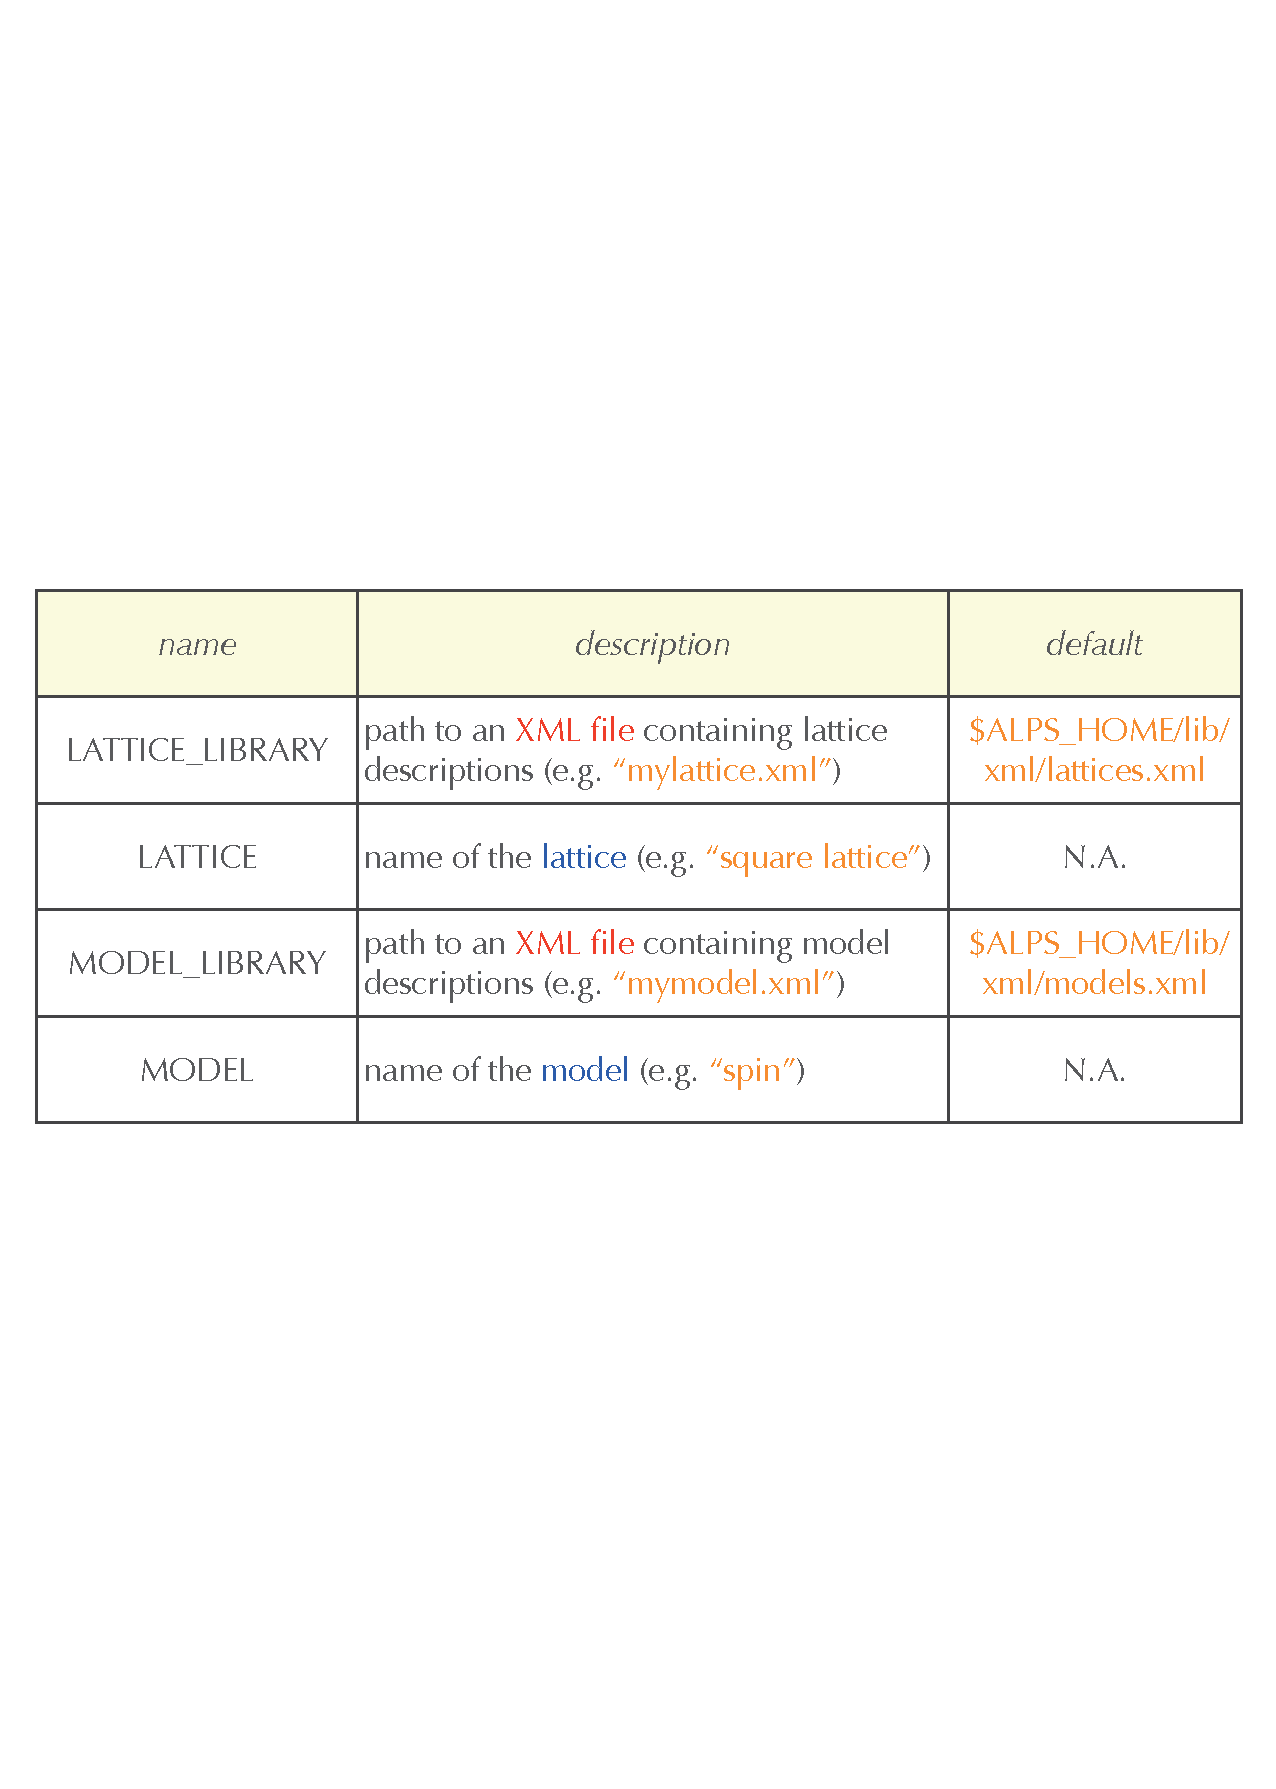
\includegraphics[height=4.5cm]{simulation5.pdf}
  \end{center}
  \end{itemize}
\end{frame}

\section{ALPSアプリケーションの実行}

\subsection*{\redm\whiteb\greenb}
\begin{frame}[t,fragile]{ALPSアプリケーションの実行方法}
  \begin{enumerate}
  \item Pythonスクリプトから: 例) \href{https://github.com/cmsi/alps-tutorial/blob/tutorials/tutorials/mc-02-susceptibilities/tutorial2a.py}{tutorial2a.py}
    \includegraphics[height=.08\textheight]{tutorial2a-2.pdf}
  \item コマンドラインから
\begin{lstlisting}
$ spinmc --Tmin=5 param2a.in.xml
\end{lstlisting}
  \item parallel (MPI) execution (parameter parallelization)
\begin{lstlisting}
$ mpirun -np 8 spinmc --Tmin=5 --mpi param2a.in.xml
\end{lstlisting}
  \end{enumerate}
\end{frame}

\section{結果のプロット}

\subsection*{\redm\whiteb\greenb}
\begin{frame}[t,fragile]{シミュレーション結果のプロット}
  \includegraphics[height=.5\textheight]{tutorial2a-3.pdf}
  \begin{itemize}
  \item ターミナルから一行ずつ実行する場合、{\color{red}\tt ipython}が便利(tab補完、コマンド履歴など)
  \item {\color{red}\tt plt.ion()}を使うとコマンドの結果が図にすぐに反映される
  \end{itemize}
\end{frame}

\subsection*{\redm\whiteb\greenb}
\begin{frame}[t,fragile]{測定物理量の一覧の取得}
  \begin{enumerate}
    \setlength{\itemsep}{1em}
  \item \href{http://alps.comp-phys.org/mediawiki/index.php/ALPS_2_Documentation:Overview}{ALPS applications reference documentation}: 例)
    \begin{itemize}
    \item spinmc: {\footnotesize \href{http://alps.comp-phys.org/mediawiki/index.php/Documentation:ClassicalMCSimulations}{http://alps.comp-phys.org/mediawiki/in...}}
    \item loop: {\footnotesize \href{http://exa.phys.s.u-tokyo.ac.jp/en/projects/alps-looper}{http://exa.phys.s.u-tokyo.ac.jp/en/p...}}
    \end{itemize}
  \item Pythonスクリプトによる一覧の取得: 例) \href{https://gist.github.com/wistaria/71cb8d7a22f45bfe256d}{list-measurements.py}
    \lstset{language={Python},basicstyle=\small}
\begin{lstlisting}
import pyalps
data = pyalps.loadMeasurements(
       pyalps.getResultFiles(prefix='parm2c'))
{ item.props['observable'] for item in pyalps.flatten(data) }
\end{lstlisting}
  \item (上級者向け) h5dumpユーリティティを利用して *.h5 ファイルの中を見る
  \end{enumerate}
\end{frame}

\section{ALPSの実行シナリオ}

\subsection*{\redm\whiteb\greenb}
\begin{frame}[t,fragile]
  \frametitle{ALPSの実行シナリオ}
  \begin{enumerate}
  \item コマンドライン
\begin{lstlisting}
$ parameter2xml param
$ loop param.in.xml
\end{lstlisting}
  \item シェルスクリプト(バッチ処理)
  \item Python (対話的 or バッチ)
    \begin{itemize}
    \item パラメータの準備からグラフ作成まで統一的に
    \item 対話的にもバッチコマンドとしても実行可能
    \item グラフの作成も、PythonのMatplotlibを用いる
    \end{itemize}
  \item IPython notebook
    \begin{itemize}
    \item ブラウザ上でPythonコマンドを実行
    \item 入力、出力を「ノートブック」としてまとめて保存
    \item グラフの描画もブラウザ上で可能
    \end{itemize}
  \item VisTrails (履歴管理ツール)
  \end{enumerate}
\end{frame}

\subsection*{\redm\whitem\greenb}
\begin{frame}[t,fragile]
  \frametitle{コマンドライン実行 (厳密対角化 ed-01)}
  \begin{enumerate}
  \item ワークステーションにログイン
\begin{lstlisting}
$ ssh -YC username@hostname
\end{lstlisting}
  \item 環境変数のセットアップ
\begin{lstlisting}
$ source /somewhere/alpsvars.sh
\end{lstlisting}
  \item 入力XMLファイルの準備
\begin{lstlisting}
$ cd tutorials/ed-01-sparsediag
$ parameter2xml parm1a
\end{lstlisting}
  \item sparsediagの実行
\begin{lstlisting}
$ sparsediag --write-xml parm1a.in.xml
\end{lstlisting}
  \item 結果はparm1a.task1.out.xmlに出力される
  \end{enumerate}
\end{frame}

\subsection*{\redm\whitem\greenb}
\begin{frame}[t,fragile]
  \frametitle{シェルスクリプトによる実行 (厳密対角化 ed-01)}
  \begin{enumerate}
  \item ワークステーションにログイン
\begin{lstlisting}
$ ssh -YC username@hostname
\end{lstlisting}
  \item シェルスクリプト(バッチファイル)の準備
\begin{lstlisting}
$ cd tutorials/ed-01-sparsediag
$ vi batch.sh
\end{lstlisting}
  \item batch.sh の中身
\lstset{language={bash}}
\begin{lstlisting}
#!/bin/sh
source /somewhere/alpsvars.sh
parameter2xml parm1a
sparsediag --write-xml parm1a.in.xml
\end{lstlisting}
  \item シェルスクリプトを実行 (あるいはバッチキューに投入)
  \item 物性研スパコンでのジョブスクリプトの書き方 ⇒ \href{http://www.issp.u-tokyo.ac.jp/supercom/for-users/x92nxz/alps}{[LINK]}
  \end{enumerate}
\end{frame}

\subsection*{\redm\whitem\greenb}
\begin{frame}[t,fragile]
  \frametitle{Pythonでの対話的実行 (厳密対角化 ed-01)}
  \begin{enumerate}
  \item ワークステーションにSSHログイン
\begin{lstlisting}
$ ssh -YC username@hostname
\end{lstlisting}
  \item 環境変数のセットアップ
\begin{lstlisting}
$ source /somewhere/alpsvars.sh
\end{lstlisting}
  \item IPythonの起動
\begin{lstlisting}
$ cd tutorials/ed-01-sparsediag
$ ipython
\end{lstlisting}
  \item \href{http://alps.comp-phys.org/mediawiki/index.php/ALPS_2_Tutorials:ED-01_SparseDiagonalization/ja#Python.E3.81.A7.E3.81.AE.E5.AE.9F.E8.A1.8C}{チュートリアルページ}にしたがって、コマンドを実行 (コマンドはTABで補完できる)
  \end{enumerate}
\end{frame}

\subsection*{\redm\whitem\greenb}
\begin{frame}[t,fragile]
  \frametitle{Pythonでのバッチ実行 (厳密対角化 ed-01)}
  \begin{enumerate}
  \item ワークステーションにSSHログイン
\begin{lstlisting}
$ ssh -YC username@hostname
\end{lstlisting}
  \item 環境変数のセットアップ
\begin{lstlisting}
$ source /somewhere/alpsvars.sh
\end{lstlisting}
  \item バッチ実行
\begin{lstlisting}
$ cd tutorials/ed-01-sparsediag
$ python tutorial1a.py
\end{lstlisting}
  \end{enumerate}
\end{frame}

\subsection*{\redm\whitem\greenb}
\begin{frame}[t,fragile,shrink=10]
  \frametitle{IPython notebookでの実行 (厳密対角化 ed-01)}
  \begin{enumerate}
  \item ワークステーションにSSHログイン
\begin{lstlisting}
$ ssh -YC username@hostname
\end{lstlisting}
  \item IPython notebookサーバの起動
\begin{lstlisting}
$ source /somewhere/alpsvars.sh
$ cd notebook/jp
$ ipython notebook --no-browser --pylab inline
\end{lstlisting}
  \item 起動時に出力されるポート番号(8888等)を控えておく
  \item 手元のPCでもう一つポートフォワーディング付きでSSHセッションを開く
\begin{lstlisting}
$ ssh username@hostname -L 8888:localhost:8888
\end{lstlisting}
  \item PCでブラウザを起動し、http://localhost:8888 を開く
  \item ED-01\_SparseDiagonalization.ipynb を開き、[Shift+Return] で実行していく
  \end{enumerate}
\end{frame}

\subsection*{\redm\whitem\greenb}
\begin{frame}[t,fragile]
  \frametitle{IPython notebookでの実行 (ローカル環境を使う場合)}
  \begin{itemize}
    \setlength{\itemsep}{1em}
  \item IPython notebookの起動
\begin{lstlisting}
$ source $HOME/alps/alpsvars.sh
$ cd notebook/jp
$ ipython notebook --pylab inline
\end{lstlisting}
  \item Mac OS X の場合は, {\tt ipython-2.7}を使う
  \item MateriApps LIVE!の場合は, 1行目は不要
  \end{itemize}
\end{frame}

\subsection*{\redm\whitem\greenb}
\begin{frame}[t,fragile]{シミュレーションの並列実行}
  \begin{itemize}
    \item パラメータセットに関する並列実行が可能 (embarassingly parallel)
    \item アプリケーションによって、ALPS parallelizing スケジューラか、ALPS/parapack スケジューラのいずれかが使われている (オプション -l により確認可)
    \item ALPS parallelizing スケジューラ (spinmc等)
      \begin{itemize}
        \item OpenMPスレッド並列には対応していない。MPI並列のみ
        \item MPI実行例(4プロセス): \\ {\tt {\color{red} mpirun -np 4} spinmc {\color{red} --mpi} parm2a.in.xml}
      \end{itemize}
    \item ALPS/parapack スケジューラ (loop等)
      \begin{itemize}
        \item OpenMPスレッド並列とMPI並列に対応。デフォルトで自動的にスレッド並列実行
        \item 実行例(16スレッド): \\ {\tt loop {\color{red} -r 16} parm2c.in.xml}
      \end{itemize}
  \end{itemize}
\end{frame}

\subsection*{\redm\whitem\greenb}
\begin{frame}[t,fragile]{実行結果の確認}
  \begin{itemize}
    \item 実行結果(JOB XMLファイル、TASK XMLファイル)は、webブラウザで直接開いて中身を確認することも可能
      \begin{itemize}
      \item 例(MateriApps LIVE!): iceweasel parm1a.task1.out.xml
      \item 例(Linux): firefox parm1a.task1.out.xml
      \item 例(Mac OS X): open -a safari parm1a.task1.out.xml
      \end{itemize}
  \end{itemize}
\end{frame}

\section{もっとチュートリアル}

\subsection*{\redm\whiteb\greenb}
\begin{frame}[t,fragile]{より高度なチュートリアル}
  \begin{itemize}
  \item パラメータファイルを変更することで、以下のようなシミュレーションが実行可能:
    \begin{itemize}
    \item 温度点の追加
    \item システムサイズの追加
    \item スピン1の鎖
    \item イジング的(容易軸的)な異方性
    \item 他の格子構造(二次元正方格子など)
    \end{itemize}
  \item ED, MC, QMC, DMRG, DMFTに関する様々なチュートリアル: \href{http://alps.comp-phys.org/mediawiki/index.php/ALPS_2_Tutorials:Overview}{ALPS Tutorials}
  \item 格子構造やハミルトニアンを自分で定義するには: \href{http://alps.comp-phys.org/mediawiki/index.php/Tutorials:LatticeHOWTO}{ALPS Lattice HowTo}、\href{http://alps.comp-phys.org/mediawiki/index.php/Tutorials:ModelHOWTO}{ALPS Model HowTo}
  \end{itemize}
\end{frame}

\subsection*{\redm\whiteb\greenb}
\begin{frame}[t,fragile]{ALPS格子チュートリアル}
  \href{http://alps.comp-phys.org/mediawiki/index.php/Tutorials:LatticeHOWTO/ja}{ALPS Lattice HowTo} \\
  \begin{itemize}
    \item \href{http://alps.comp-phys.org/mediawiki/index.php/Tutorials:LatticeHOWTO:SimpleGraphs/ja}{辺と頂点を単位として簡単なグラフを指定する方法}
    \item \href{http://alps.comp-phys.org/mediawiki/index.php/Tutorials:LatticesAndUnitCells/ja}{格子と単一セルを指定する方法}
    \item \href{http://alps.comp-phys.org/mediawiki/index.php/Tutorials:LatticesAndGraphs/ja}{単位格子に対応するグラフを指定する方法}
    \item \href{http://alps.comp-phys.org/mediawiki/index.php/Tutorials:LatticeHOWTO:Library/ja}{格子とグラフのライブラリの生成方法}
    \item \href{http://alps.comp-phys.org/mediawiki/index.php/Tutorials:LatticeHowto:CheckLattice/ja}{格子の定義から生成されたグラフを確認する方法}
  \end{itemize}
\end{frame}

\subsection*{\redm\whiteb\greenb}
\begin{frame}[t,fragile]{ALPS模型チュートリアル}
  \href{http://alps.comp-phys.org/mediawiki/index.php/Tutorials:ModelHOWTO}{ALPS Model HowTo} \\
  \begin{itemize}
  \item \href{http://alps.comp-phys.org/mediawiki/index.php/Tutorials:ModelHOWTO/ja\#.E3.83.87.E3.83.95.E3.82.A9.E3.83.AB.E3.83.88.E3.81.AE.E3.83.A2.E3.83.87.E3.83.AB.E3.83.A9.E3.82.A4.E3.83.96.E3.83.A9.E3.83.AA.E3.83.95.E3.82.A1.E3.82.A4.E3.83.AB.E3.80.80}{デフォルトのモデルライブラリファイル}
  \item \href{http://alps.comp-phys.org/mediawiki/index.php/Tutorials:ModelHOWTO/ja\#.E3.83.A2.E3.83.87.E3.83.AB.E3.83.A9.E3.82.A4.E3.83.96.E3.83.A9.E3.83.AA.E3.83.95.E3.82.A1.E3.82.A4.E3.83.AB.E3.81.AE.E6.A7.8B.E9.80.A0}{モデルライブラリファイルの構造}
  \item \href{http://alps.comp-phys.org/mediawiki/index.php/Tutorials:ModelHOWTO/ja\#.E5.8D.98.E4.B8.80.E3.82.B5.E3.82.A4.E3.83.88.E3.81.AE.E5.9F.BA.E5.BA.95}{単一サイトの基底}
  \item \href{http://alps.comp-phys.org/mediawiki/index.php/Tutorials:ModelHOWTO/ja\#.E5.AE.8C.E5.85.A8.E6.A0.BC.E5.AD.90.E3.83.A2.E3.83.87.E3.83.AB.E3.81.AE.E5.9F.BA.E5.BA.95}{完全格子モデルの基底}
  \item \href{http://alps.comp-phys.org/mediawiki/index.php/Tutorials:ModelHOWTO/ja\#.E9.87.8F.E5.AD.90.E6.BC.94.E7.AE.97.E5.AD.90}{量子演算子}
  \item \href{http://alps.comp-phys.org/mediawiki/index.php/Tutorials:ModelHOWTO/ja\#.E3.83.8F.E3.83.9F.E3.83.AB.E3.83.88.E3.83.8B.E3.82.A2.E3.83.B3.E3.81.AE.E5.8F.96.E6.89.B1.E3.81.84}{ハミルトニアンの取扱い}
  \end{itemize}
\end{frame}

\subsection*{\redm\whiteb\greenm}
\begin{frame}[t,fragile]{厳密対角化チュートリアル}
  \begin{itemize}
  \item \href{http://alps.comp-phys.org/mediawiki/index.php/ALPS_2_Tutorials:ED-01_SparseDiagonalization/ja}{ED-01 Sparse Diagonalization (Lanczos)
}

    $S=1$の量子1次元系(サイト数4)について, Lanczos法により固有値を求め, 固有値, 相関関数などを出力する.

  \item \href{http://alps.comp-phys.org/mediawiki/index.php/ALPS_2_Tutorials:ED-02_Gaps/ja}{ED-02 Spin gaps of 1D quantum systems}
    
    $S=1$の量子1次元系(サイト数4--14)について, Lanczos法で固有値計算を行う. 求めたエネルギー固有値からエネルギーギャップを求めプロットする.

  \item \href{http://alps.comp-phys.org/mediawiki/index.php/ALPS_2_Tutorials:ED-03_Spectra/ja}{ED-03 Spectra of 1D quantum systems}

    次の2種類の量子格子模型について, Lanczos法で固有値計算を行う.
    \begin{itemize}
      \item $S=1/2$量子1次元ハイゼンベルグ模型
      \item $S=1/2$はしご格子ハイゼンベルグ模型
    \end{itemize}
  \end{itemize}
\end{frame}

\subsection*{\redm\whiteb\greenm}
\begin{frame}[t,fragile]{厳密対角化チュートリアル}
  \begin{itemize}
  \item \href{http://alps.comp-phys.org/mediawiki/index.php/ALPS_2_Tutorials:ED-04_Criticality/ja}{ED-04 Conformal field theory description of 1D critical spectra}

    横磁場イジング模型について, Lancos 法を用いた固有値計算を行う. 相関関数の臨界指数とエネルギーギャップとの共形場理論から導かれる関係を数値計算から求めた固有値により実証する.

  \item \href{http://alps.comp-phys.org/mediawiki/index.php/ALPS_2_Tutorials:ED-05_ED_Phase_Transition/ja}{ED-05 Phase transition in a frustrated spin chain}

    次近接相互作用をもつハイゼンベルグ鎖について, Lanczos法を用いて固有値計算を行う. 得られたエネルギー固有値から臨界点を求める. さらに共形場理論を利用した解析も行う.

  \item \href{http://alps.comp-phys.org/mediawiki/index.php/ALPS_2_Tutorials:ED-06_FullDiagonalization/ja}{ED-06 Full Diagonalization}

    $S=1$の反強磁性ハイゼンベルグ鎖(8サイト)について全対角化を行う. 得られた固有値をもとにいくつかの物理量について熱力学的振る舞いをプロットする.
  \end{itemize}
\end{frame}

\subsection*{\redm\whiteb\greenm}
\begin{frame}[t,fragile]{モンテカルロ法チュートリアル}
  \begin{itemize}
  \item mc-01-autocorrelations
  \item mc-01b-equilibration-and-convergence
  \item mc-02-susceptibilities
  \item mc-03-magnetization
  \item mc-04-measurements
  \item mc-05-bosons
  \item mc-06-qwl
  \item mc-07-phase-transition
  \item mc-08-quantum-phase-transition
  \end{itemize}
\end{frame}

\end{document}
